\chapter{Introduction}\label{introduction}

Bird flocking is a natural phenomenon which always appears in group activities like collective hunting, entertainment or migration. Biologists have found that the flocking behavior benefits the entire colony by improving the overall foraging~\cite{Foraging}, predators spotting~\cite{Predator} and propagation~\cite{Propagation} efficiencies. Specifically, the allocation of individual tasks, communication and motion control of each agent have determined the main characteristics of the flock system, such as the scalability, robustness and convergence rate. Missions like remote transportation, surveillance and rescue with UAVs require the agents to be fully autonomous, fault tolerant and intelligent that they could dynamically interact with the environments and local neighbors. Studies regarding the motion control and the realization of flocking with mobile robots will greatly inspire the human beings on resolving the aforementioned tasks.

Three important criteria were first studied in~\cite{Reynolds1987} to determine a stable flocking system: separation, cohesion and alignment. Alignment criterion requires each agent to match self's velocity with neighboring flockmates in the mid range, separation criterion requires each agent to repel neighboring flockmates in the short range and cohesion criterion requires each agent to steer neighboring flockmates in the long range. $\psi_{angle}$ (\ref{eq:psi_scal}) is defined to describe the convergence of agents' velocities in angle, where $k$ is the total number of agents and $\psi_{angle}$ goes to one when all agents' velocities converge to a common direction.

\begin{equation}\label{eq:psi_scal}
\psi_{angle}(t)=\frac{1}{k(k-1)}\sum^k_{i=1}\sum_{j\neq i}\frac{v_i(t)v_j(t)}{|v_i(t)||v_j(t)|}
\end{equation}

To better control the individual agents and realize the flocking system, quadrotors or UAVs are selected owing to their flexibility and mobility in 3D space. Today, the capability of a single UAV has been increasing rapidly, accompanied by the falling prices and improving performance of the communication, sensing and processing hardwares. Meanwhile, the measurement and control methods of UAVs in the flock realization are expected to be distributed. Realization with distributed measurement method requires all the information to be collected by on-board sensors, such as LiDAR, inertial measurement unit (IMU) or camera instead of external absolute positioning systems like GPS~\cite{Vicsek2018}, motion capture system (VICON)~\cite{Swarm2018,MPC} or real-time kinematic system (RTK). Realization with distributed control method requires each UAV to decide its movement with information available at that agent~\cite{MAV2017} instead of executing commands from a central computer~\cite{CAPT,POMDP,Kumar2018} or a leader UAV. The assumption of distributed architectures agrees with the nature that individual agents react to their sensed local environment and surrounding neighbors.

UAV formations~\cite{Virtual2008,LQR2014,VirtualLeader,Askari2015,Bearing2016,RAS} are often discussed with flockings~\cite{Zhang2018,Martin2014,Vicsek2018,VLAP,Behavior2004} since their cluster-like performances are very similar, however, they are distinct in several aspects. The formation problem emphasizes the relative positions~\cite{Virtual2008,LQR2014,VirtualLeader}, displacements~\cite{Askari2015,Bearing2016} or distances~\cite{RAS} between any two agents to be fixed, while the flocking problem focuses more on the coordination of all agents instead of preserving a rigid shape. The flocking model's fault tolerance ability outperforms that of formation model. The adding or removing one agent from the flocking model will not affect its stability, however, the formation will not exist if one agent is removed. From application side, the control and measurement methods of formation problems are mostly centralized and for agents in the formation model, their final stable states are independent of their initial conditions. On the contrary, the control and measurement methods of flocking problems are expected to be distributed and the final stable states of agents in flocking model depend on the initial conditions.

The gap between the simulation and the realization of the flocking models comes from two sides, the design of the model and the design of the UAV platform. From the theoretical side, first, the convergence rate of agents' velocities in flocking model is expected to be fast to prevent collisions between agents. Second, the inter-agent distance of any two agents in stable state shall live within an appropriate range that the lower and upper bounds have to be addressed due to safety and sensors' limited operating range reasons. Third, the control algorithm has to be distributed that only relative information could be used. From the experimental side, first, the control and measurement methods have to be distributed that each UAV could only use on-board sensors to percept the local environment, analyse and make decisions instead of relying on external sensors (indoor motion capture system or outdoor GPS) or centralized computer. Second, the on-board sensor is capable of measuring relative displacements. Third, camera is preferred to be the on-board sensor to maximally imitate natural birds.

\begin{figure}[htb]
  \centering
  \subfigure[Indoor environment.]{\label{fig:indoor}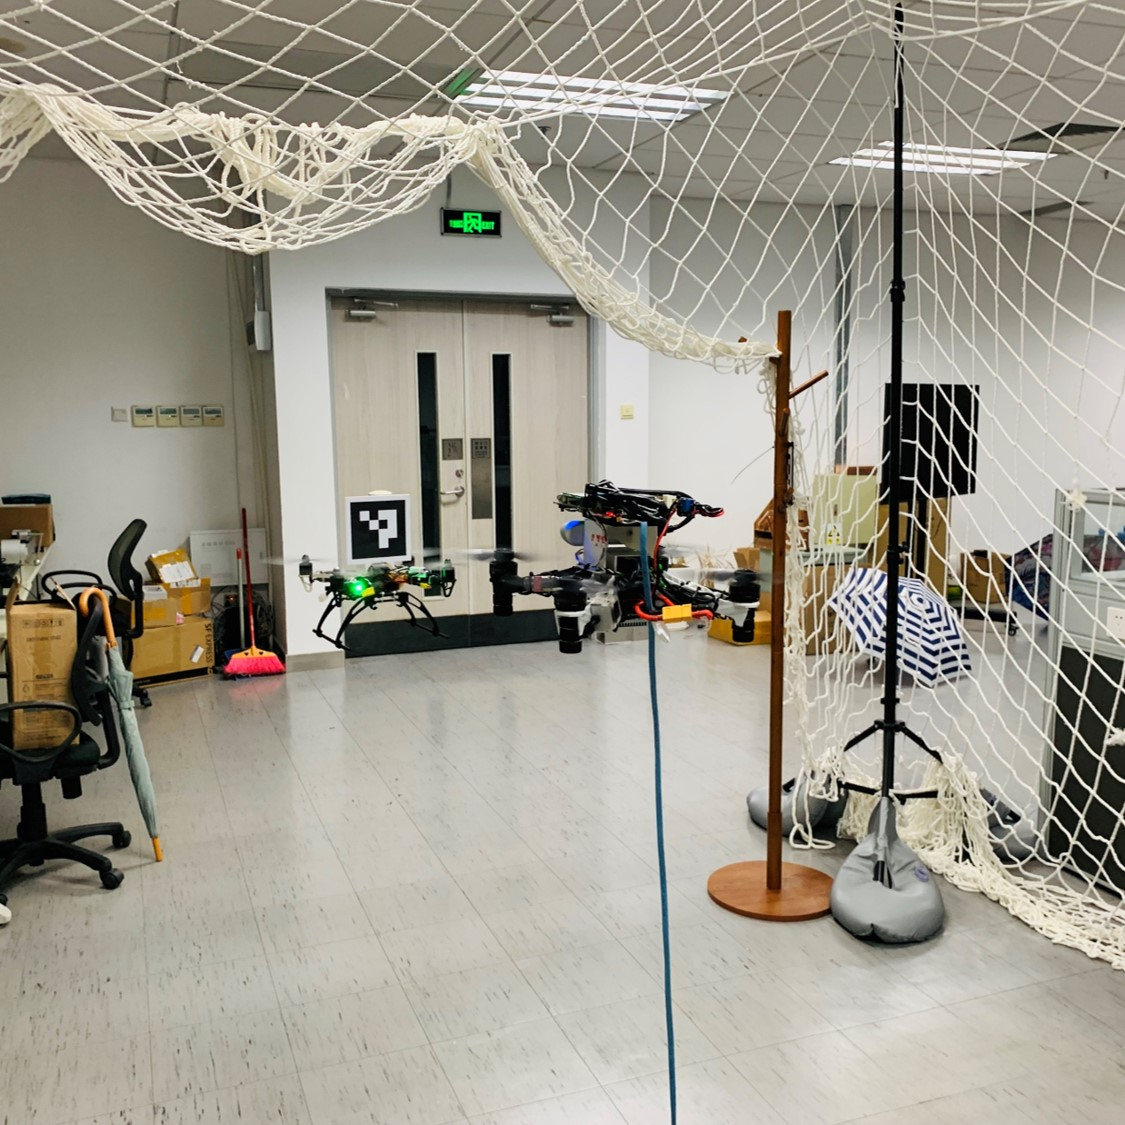
\includegraphics[width=0.49\textwidth]{figure/chapter_1/indoor.jpg}}
  \subfigure[Outdoor environment.]{\label{fig:outdoor}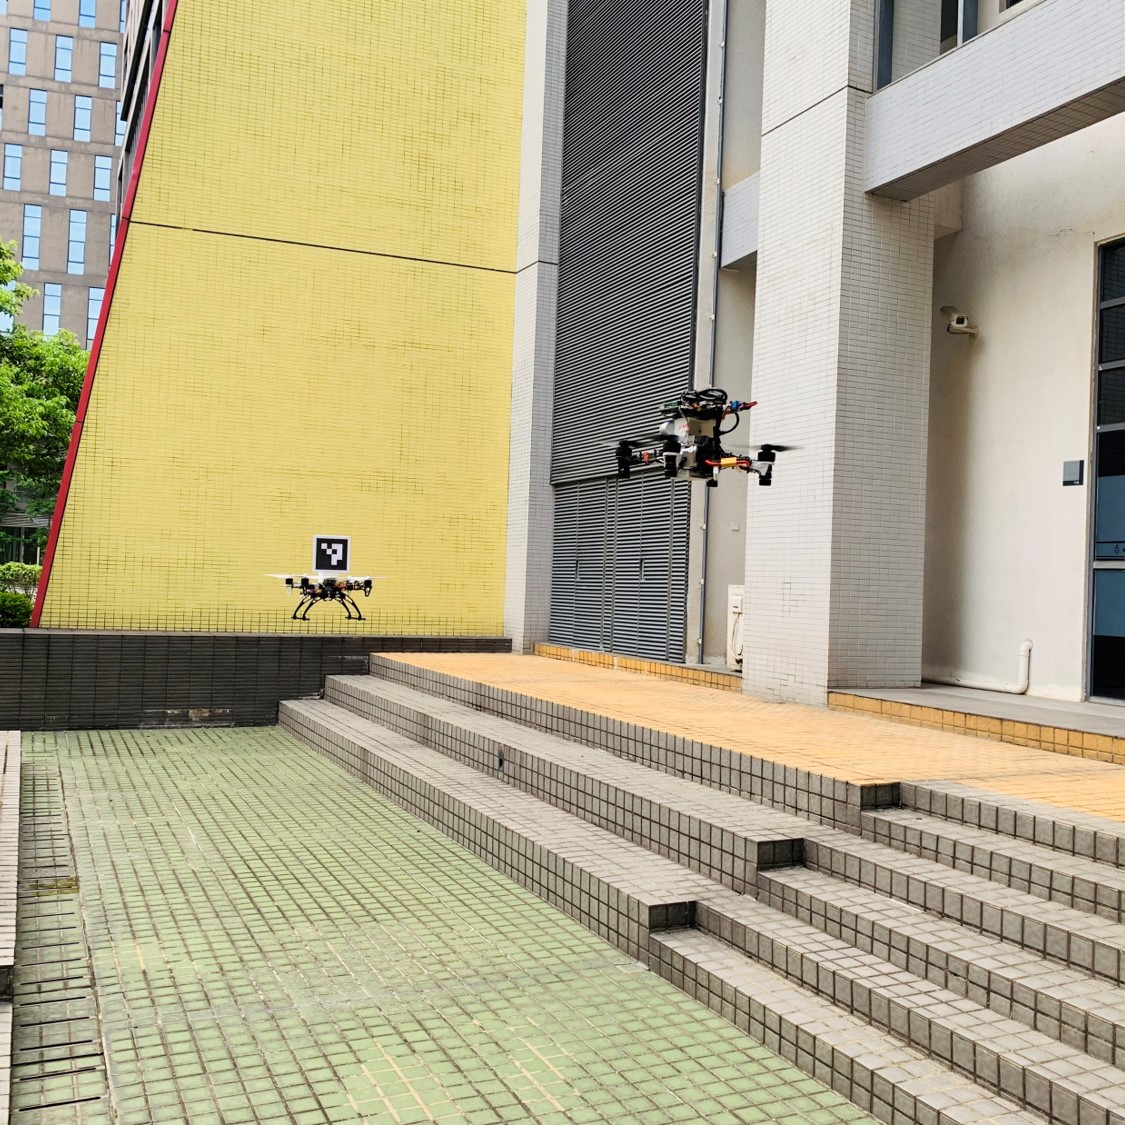
\includegraphics[width=0.49\textwidth]{figure/chapter_1/outdoor.jpg}}
  \caption{Flocking of two UAVs in GPS-denied environments. A video of the experiments can be found at \text{https://youtu.be/lIJ\_8VM-yS0.}}\label{fig:indoor_outdoor}
\end{figure}

In this thesis, we present a complete system-level solution to address the aforementioned challenges. The theoretical contribution is the proposal and the proof of a control law satisfying the three flocking criteria. The application-level contribution is the design, control and the implementation of the control law using two UAVs, with the front one being controlled manually and the latter one being fully autonomous as shown in Fig.~\ref{fig:indoor_outdoor} and Fig.~\ref{fig:twin}. We use the monocular camera as our only on-board sensor for both state estimation and target recognition to maximally imitate natural birds. The flight tests are conducted in both indoor and outdoor environments, and it is successfully demonstrated that our autonomous UAV is able to stay flocking with the proposed control law.

\begin{figure}[H]
  \centering
  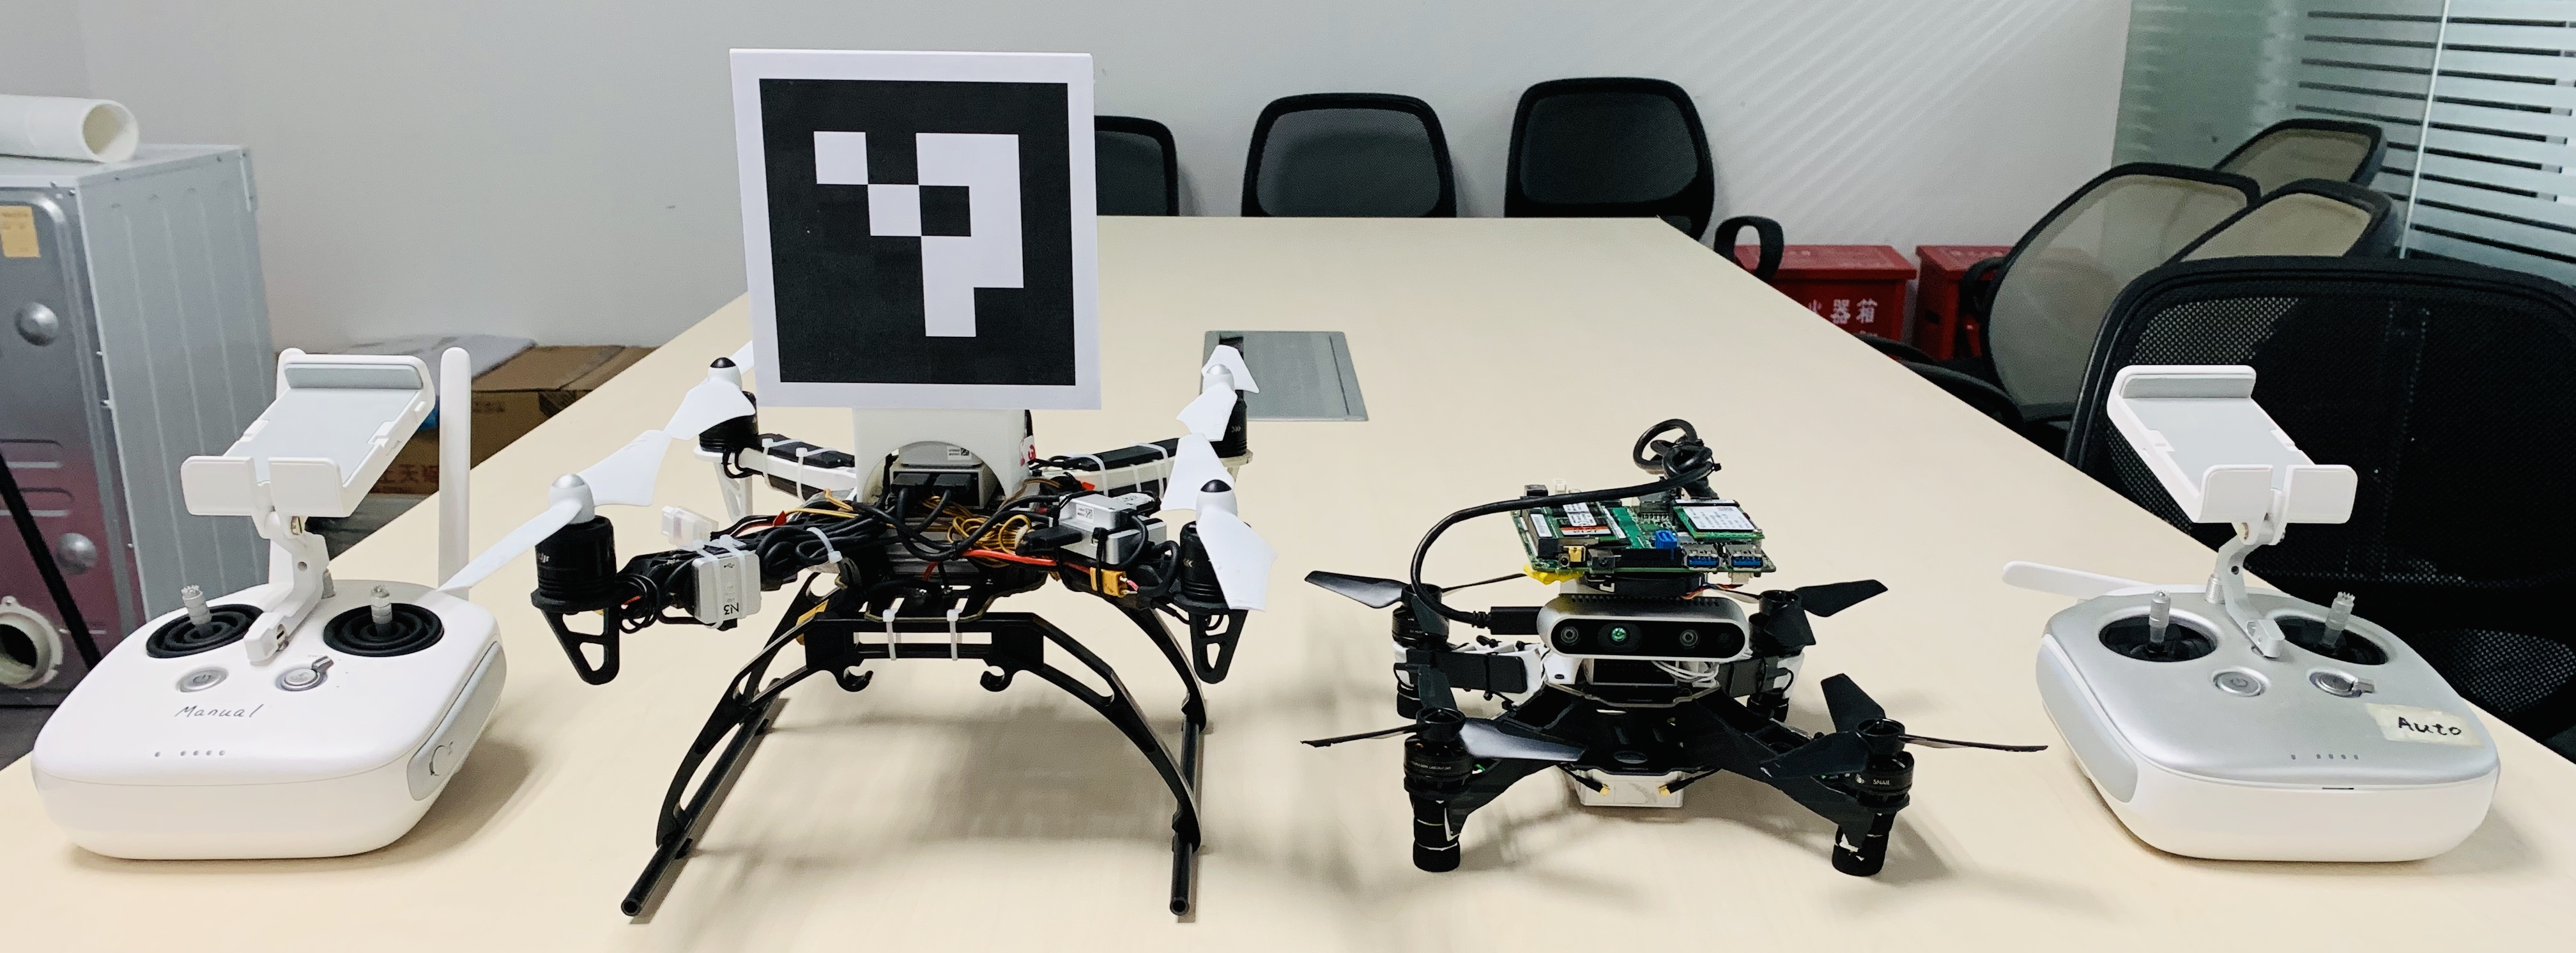
\includegraphics[width=1\textwidth]{figure/chapter_1/all.jpg}
  \caption{Our complete flocking system: the left one (leader) is manually controlled and the right one (follower) is fully autonomous.}
  \label{fig:twin}
\end{figure}

The outline of the thesis is as follows, Ch.~\ref{preliminaries} reviews the origin and some typical approaches of the flocking related consensus problem. Our proposed control model and its stability and convergence analysis are shown in Ch.~\ref{design}. Ch.~\ref{implementation} discusses the architecture and the implementation of our hardware and software platforms. Simulations and real world experiments are demonstrated in Ch.~\ref{experiment}. Ch.~\ref{conclusion} summarises this work and points out our possible improvements and future plans.

\newpage
